\documentclass[10pt,a4paper]{article}
\usepackage[margin=1.5cm,top=1.1cm,bottom=1.1cm]{geometry}
\usepackage[utf8]{inputenc}
\usepackage[T1]{fontenc}
\usepackage{lmodern}
\usepackage{microtype}
\usepackage{amsmath}
\usepackage{caption}
\usepackage{tikz}
\usetikzlibrary{arrows.meta,positioning,shapes.geometric,fit,backgrounds,calc}
\usepackage[hidelinks]{hyperref}
\usepackage{titlesec}
\titlespacing*{\section}{0pt}{5pt}{2pt}
\titleformat{\section}{\normalsize\bfseries}{\thesection}{0.6em}{}
\setlength{\parskip}{1.5pt}
\setlength{\parindent}{10pt}
\captionsetup{font=small,skip=3pt}
\pagestyle{empty}

\title{\vspace{-16pt}\Large\textbf{pi-billboard: Audience-Aware Digital Signage on a Raspberry Pi}\vspace{-4pt}}
\author{\normalsize Dilan Perera \quad\textit{ISMR Labs}\\[-2pt]\small\url{https://github.com/ISMR-Labs/pi-billboard}}
\date{\vspace{-8pt}\small October 2026\vspace{-14pt}}

\begin{document}
\maketitle\thispagestyle{empty}

\begin{abstract}
\noindent
Digital billboards usually play a fixed loop regardless of who is watching. \emph{pi-billboard} is a
self-contained signage platform that runs entirely on a Raspberry Pi with a camera. Ads are uploaded into
categories through a web dashboard; during playback the camera counts the people in front of the screen and,
from a lightweight head-pose estimate, how many of them are looking at it. The attention rate of each category
(lookers\,/\,viewers) drives a Thompson-sampling scheduler with time decay, so the screen converges on the
content its current audience responds to while still exploring. No cloud service, GPU or identity data is
needed: only counts leave the camera thread. The two vision models total under 5\,MB and run at 5--8\,fps on a Pi~4.
\end{abstract}
\vspace{-4pt}

\section{Introduction}
Attention is the scarce resource in out-of-home advertising, yet small-scale signage cannot measure it and
therefore cannot act on it. Commercial audience-measurement products depend on cloud analytics, dedicated
hardware or face recognition, which raises cost and privacy concerns. Our goal was a system a shop, lab or
campus can deploy on a \$50 computer, that keeps all processing on the device, and that \emph{closes the loop}:
measurement changes what is played instead of only producing a report.

The platform makes three contributions. (1)~An on-device audience sensor that separates \emph{presence} from
\emph{attention} by estimating head orientation relative to the screen. (2)~A tracker that turns per-frame
detections into per-person counts, so a viewer is counted once per ad rather than once per frame. (3)~A
scheduler that treats the choice of category as a multi-armed bandit, handling the explore/exploit trade-off
and a non-stationary audience (lunch crowd versus evening crowd) in a principled way. Around this sit the
practical parts: upload and categorisation of image and video ads, dayparting, a live dashboard with per-ad and
per-category statistics, and a kiosk player for the display (Fig.~\ref{fig:arch}).

\section{Methodology}

\begin{center}
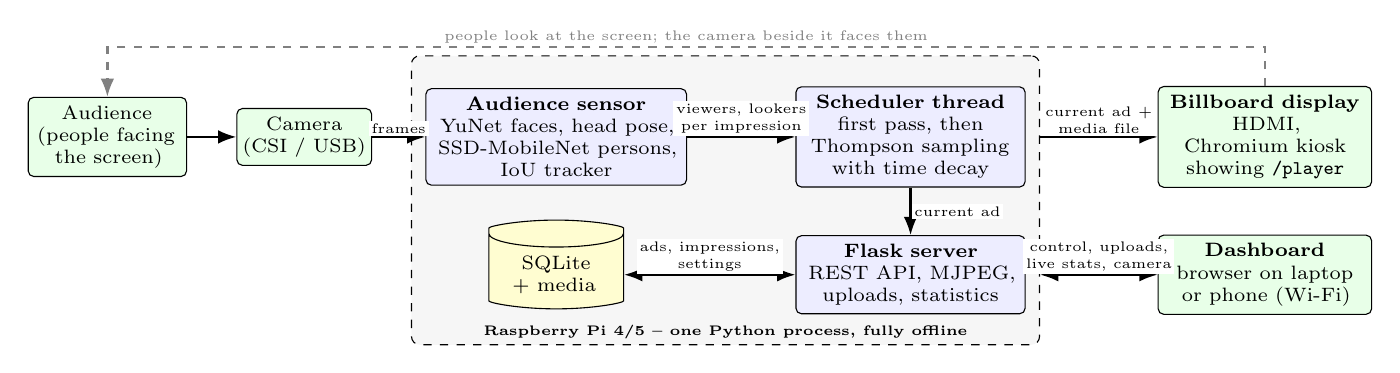
\begin{tikzpicture}[
  font=\scriptsize, >=Latex, x=1cm, y=1cm,
  box/.style={draw, rounded corners=2pt, align=center, inner sep=3pt, minimum height=16pt, fill=white},
  comp/.style={box, fill=blue!7},
  ext/.style={box, fill=green!9},
  store/.style={box, cylinder, shape border rotate=90, aspect=0.2, fill=yellow!18, minimum height=20pt},
  flow/.style={->, thick},
  lbl/.style={font=\tiny, fill=white, inner sep=1pt, align=center}
]
\node[ext, text width=1.8cm] (people) at (0,0) {Audience\\(people facing\\the screen)};
\node[ext, text width=1.5cm] (cam) at (2.5,0) {Camera\\(CSI / USB)};
\node[comp, text width=3.1cm] (sensor) at (5.7,0) {\textbf{Audience sensor}\\YuNet faces, head pose,\\SSD-MobileNet persons,\\IoU tracker};
\node[comp, text width=2.7cm] (sched) at (10.2,0) {\textbf{Scheduler thread}\\first pass, then\\Thompson sampling\\with time decay};
\node[store, text width=1.5cm] (db) at (5.7,-1.75) {SQLite\\+ media};
\node[comp, text width=2.7cm] (server) at (10.2,-1.75) {\textbf{Flask server}\\REST API, MJPEG,\\uploads, statistics};
\begin{scope}[on background layer]
\node[draw, dashed, rounded corners=3pt, fill=gray!7, fit=(sensor)(sched)(db)(server), inner xsep=5pt, inner ysep=11pt] (pi) {};
\end{scope}
\node[font=\tiny\bfseries, anchor=south, inner sep=2pt] at (pi.south) {Raspberry Pi 4/5 -- one Python process, fully offline};
\node[ext, text width=2.5cm] (display) at (14.7,0) {\textbf{Billboard display}\\HDMI, Chromium kiosk\\showing \texttt{/player}};
\node[ext, text width=2.5cm] (dash) at (14.7,-1.75) {\textbf{Dashboard}\\browser on laptop\\or phone (Wi-Fi)};
\draw[flow] (people) -- (cam);
\draw[flow] (cam) -- node[lbl, above]{frames} (sensor);
\draw[flow] (sensor) -- node[lbl, above]{viewers, lookers\\per impression} (sched);
\draw[flow] (sched) -- node[lbl, right]{current ad} (server);
\draw[flow, <->] (server) -- node[lbl, above]{ads, impressions,\\settings} (db);
\draw[flow] (pi.east |- display.west) -- node[lbl, above]{current ad +\\media file} (display.west);
\draw[flow, <->] (pi.east |- dash.west) -- node[lbl, above]{control, uploads,\\live stats, camera} (dash.west);
\draw[flow, dashed, gray] (display.north) -- ++(0,0.5) -| node[lbl, pos=0.25, above, text=gray]{people look at the screen; the camera beside it faces them} (people.north);
\end{tikzpicture}
\vspace{2pt}
\captionof{figure}{Overall architecture. The camera sits beside the display and faces the audience; the display is
a browser in kiosk mode that polls the server for the current ad. Everything runs offline on the Pi.}
\label{fig:arch}
\end{center}
\vspace{-6pt}

\textbf{Audience sensing.} Each frame is processed by two small models: YuNet (OpenCV, 230\,KB) returns face
boxes with five landmarks, and a quantised SSD-MobileNet~v1 (TFLite, 4\,MB, run every third frame) returns
person boxes so that people facing away are still counted. From the five landmarks we solve a
perspective-$n$-point problem against a generic 3-D face model to obtain the head's rotation $R$ and
translation $t$ in camera coordinates. The attention angle is $\theta=\arccos(\hat f\cdot\hat c)$ with
$\hat f=R\,[0,0,-1]^{\top}$ the head's forward direction and $\hat c=-t/\lVert t\rVert$ the direction from the
head to the camera; a face is \emph{looking} when $\theta<25^{\circ}$. Using the direction to the camera rather
than raw yaw classifies a person at the edge of the frame who turns toward the screen correctly. Faces are
merged into person boxes by containment and a greedy IoU tracker assigns stable ids. During an ad play (an
\emph{impression}) a track is a \emph{viewer} if present for $\geq 0.5$\,s and a \emph{looker} if it faced the
screen for $\geq 0.7$\,s, giving per-person rather than per-frame counts.

\textbf{Scheduling.} Let category $c$ have $v_{c,i}$ viewers and $\ell_{c,i}$ lookers in its past impression
$i$. We keep a Beta belief over its attention rate,
$p_c\sim\mathrm{Beta}\big(1+\sum_i w_i\,\ell_{c,i},\;1+\sum_i w_i\,(v_{c,i}-\ell_{c,i})\big)$, with
$w_i=2^{-(t_{\text{now}}-t_i)/h}$ discounting old impressions by a half-life $h$ (default 2\,h) so the belief
follows a changing audience. When playback starts, one ad from every category is shown. Thereafter, before each
slot, a sample $\tilde p_c$ is drawn per category and the arg-max is played (Thompson sampling); with
probability $\varepsilon=0.1$ a random category is played so none starves. The same sampling picks the ad
within the category, excluding the one that just played. Impressions with no viewers do not update the belief,
and categories added at runtime get an immediate first play.

\textbf{Platform.} A Flask server with SQLite exposes a REST API, an MJPEG camera stream, a dashboard
(categories, uploads, start/stop/skip, per-ad and per-category plays, viewers, lookers, attention and current
belief, hourly chart, CSV export) and the player page that Chromium shows fullscreen on the Pi's HDMI output.
Media and data stay on the Pi, no internet access is required, and playback resumes after a reboot.

\end{document}
